\documentclass[11pt,a4paper]{article}

\usepackage{fontspec}
\usepackage[czech]{babel}
\defaultfontfeatures{Ligatures=TeX}
\setmainfont{Latin Modern Roman}
\setsansfont{Latin Modern Sans}
\setmonofont{Latin Modern Mono}

\usepackage[unicode,colorlinks=true,linkcolor=black,citecolor=blue,urlcolor=blue]{hyperref}

\usepackage{amsfonts,amsmath}
\usepackage{booktabs}
\usepackage{calc}
\usepackage{caption}
\usepackage{csquotes}
\usepackage{etoolbox}
\usepackage{float}
\usepackage{geometry}
\usepackage{graphicx}
\usepackage{listings}
\usepackage{pdfpages}
\usepackage{setspace}
\usepackage{subcaption}
\usepackage{titlesec}
\usepackage{xcolor}
\usepackage[
  backend=biber,
  style=authoryear,
  sorting=nyt,
  giveninits=true,
  uniquename=init,
  maxcitenames=2,
  doi=true,
  url=true,
  isbn=false,
  eprint=false
]{biblatex}

\geometry{
  verbose,
  tmargin=4cm,
  bmargin=3cm,
  lmargin=2.5cm,
  rmargin=2.5cm,
  footskip=24pt
}

\setcounter{secnumdepth}{3}
\setlength{\headheight}{14pt}
\setlength{\parindent}{0pt}
\setlength{\parskip}{0.8\baselineskip}

\newcommand{\tacrlogo}{resources/zprávy/za 2025/logo_TACR_zakl.pdf}

\usepackage{fancyhdr}
\pagestyle{fancy}
\renewcommand{\headrulewidth}{0pt}
\fancyhead[L]{\begin{picture}(0,0)
\put(0,0){\includegraphics[width=2cm]{\tacrlogo}}
\end{picture}}

\newcommand{\obraz}[1]{(viz obr.~\ref{#1})}
\newcommand{\tabul}[1]{(viz tab.~\ref{#1})}
\newcommand{\pozn}[1]{(viz odst.~\ref{#1})}
\newcommand{\todo}[1]{{\color{red}#1}}

\def\UNIT#1#2{\ifstrempty{#2}{}{\ifstrequal{#2}{1}{\mathrm{#1}}{\mathrm{#1}^{#2}}}}
\def\units#1#2#3{\ifstrempty{#1#2#3}{$[-]$}{$[ \UNIT{kg}{#1}\UNIT{m}{#2}\UNIT{s}{#3} ]$}}
\def\unitss#1#2#3{\ifstrempty{#1#2#3}{$-$}{$ \UNIT{kg}{#1}\UNIT{m}{#2}\UNIT{s}{#3} $}}

\def\abs#1{\lvert#1\rvert}
\def\argdot{{\hspace{0.18em}\cdot\hspace{0.18em}}}
\def\bb{\vc b}
\def\d{\mathrm{d}}
\def\D{{\tn D}}
\def\div{\operatorname{div}}
\def\grad{\nabla}
\def\jmp#1{[#1]}
\def\n{\vc n}
\def\nn{\vc n}
\def\prtl{\partial}
\def\R{\mathbb R}
\def\Real{\mathbb R}
\def\sc#1#2{\left(#1,#2\right)}
\def\th{\vartheta}
\def\tn#1{{\mathbb{#1}}}
\def\vc#1{\mathbf{\boldsymbol{#1}}}
\def\E{{\mathsf E}}
\def\avg#1{\langle#1\rangle}
\def\var#1{\llangle#1\rrangle}
\def\Var{\mathop{\rm Var}}
\def\Cov{\mathop{\rm Cov}}
\def\vl{{\vc\lambda}}
\def\estvl{{\vc{\hat\lambda}}}
\def\estrho{\hat\rho}
\def\vmu{\vc\mu}
\def\estvmu{{\vc{\hat\mu}}}
\def\vphi{\vc\phi}

\addbibresource{zprava.bib}

\begin{document}
\begin{onehalfspacing}

\hypersetup{pageanchor=false}
\begin{titlepage}
    \includegraphics[width=2cm]{\tacrlogo}

    \vspace{4cm}
    {\centering
      {\LARGE\bfseries Systém pro kontinuální monitoring vadózní zóny\\
      a predikci hladiny vody v hlubokých kolektorech\\
      --- Souhrnná výzkumná zpráva\par}
    }

    \vspace{2.2cm}
    {\Large
      {\noindent Číslo projektu: SS06010280\par}
      \vspace{2ex}
      {\noindent Předkládají:\par
      \-\hspace{2ex} organizace: {\bfseries Technická univerzita v Liberci}\\
      \-\hspace{2ex} řešitel: {\bfseries doc. Mgr. Jan Březina, Ph.D.}\\
      \-\hspace{2ex} organizace: {\bfseries Česká geologická služba}\\
      \-\hspace{2ex} spoluřešitel: {\bfseries Mgr. Ondřej Nol}\par}
    }

    \vfill
    {\large Liberec, 2026\par}
\end{titlepage}
\clearpage
\hypersetup{pageanchor=true}

\tableofcontents
\clearpage

\section{Úvod}
\label{sec:uvod}
Předkládaná souhrnná výzkumná zpráva shrnuje průběh a výsledky projektu
HLAVO pro potřeby Ministerstva životního prostředí. Projekt byl od počátku
zaměřen na vysvětlení poklesů hladin podzemní vody v hlubších kolektorech a
na návrh systému, který by pro vybranou lokalitu umožnil průběžně
vyhodnocovat doplňování zásob podzemní vody a následně predikovat vývoj
hladiny podzemní vody. Jako hlavní experimentální lokalita byla zvolena
Uhelná, kde je k dispozici husté hydrogeologické sledování, malá infiltrační
oblast a současně výrazná vazba mezi atmosférickými podmínkami, průsakem
vadózní zónou a stavem svrchních kolektorů.

Smyslem zprávy není jen chronologicky popsat dílčí práce partnerů, ale také
ukázat, jak na sebe navazují hydrologická motivace, měřicí infrastruktura,
numerické modelování a zpracování dat. V sekci~\ref{sec:motivace} je proto
nejprve shrnuto, proč byla za reprezentativní úlohu zvolena právě kombinace
lokality Uhelná a hlubokých vrtů v české křídové pánvi. Následující
sekce~\ref{sec:prubeh} shrnuje hlavní etapy řešení projektu, včetně
dočasného odklonu k vývoji hlubokého elektromagnetického čidla a následného
návratu k integrovanému predikčnímu systému. Sekce~\ref{sec:reserse} pak
rámcově zasazuje projekt do kontextu odborných prací o monitoringu
vlhkosti, modelování vadózní zóny a asimilaci dat.

Další části zprávy jsou věnovány vlastnímu výsledku projektu, tedy softwaru
HLAVO a funkčnímu vzorku integrace měření, datových toků a modelů. Tyto
sekce současně poskytují základní návod, jak systém chápat a jaké vstupy
jsou nutné pro jeho aplikaci na lokalitu Uhelná i na jiné lokality v rámci
České křídové tabule.

\section{Hydrologická motivace projektu}
\label{sec:motivace}
Hydrologická motivace projektu vychází ze srovnání dlouhodobých řad hladin
podzemní vody na pozorovací síti ČHMÚ a na vrtech ve svrchním kolektoru v
okolí Uhelné. Režimní sledování hladin podzemní vody má v České republice
dlouhodobou tradici s více než padesátiletými záznamy a ČHMÚ dlouhodobě
sleduje hladiny podzemní vody na více než 1250 vrtech.

Dlouhodobý vývoj hladin podzemní vody se vyznačuje různým podílem
sezónního kolísání a dlouhodobého trendu i různou rychlostí reakce na výrazné
dotační epizody. Měřené vrty jsou dále ovlivňovány vnějšími vlivy, například odběry
podzemní vody, stárnutím vrtu nebo změnou způsobu měření a vyhodnocování. V
rámci jednoho hydrogeologického rajonu se stejnými hydrogeologickými poměry se
tak nacházejí vrty s velmi odlišným kolísáním hladin podzemní vody. Analýza
hladin podzemní vody ukázala, že poměr sezónního kolísání a dlouhodobého
trendu mimo jiné závisí na hloubce vystrojení vrtu, hloubce hladiny podzemní
vody a často i na vzdálenosti od výrazného povrchového toku.

Z následujícího popisu chování hladin podzemní vody byly vyloučeny vrty s
neinterpretovatelným chováním hladiny podzemní vody a dlouhodobě ovlivněné
vrty čerpáním podzemní vody, kam například patří nejhlubší vrty v
cenomanském kolektoru.

\subsection{Typové režimy kolísání hladin podzemní vody}
\subsubsection{Vrty v kvartérních hydrogeologických rajonech}
Vrty v kvartérních hydrogeologických rajonech se vyznačují velmi výrazným
sezónním kolísáním, na kterém je patrný dlouhodobý trend \obraz{fig:motivace-kvart}.
V historickém záznamu hladin podzemní vody jsou velmi zřetelná období s
výrazně nižšími hladinami podzemní vody v letech 1973--1974, 1983--1984,
1990--1994 a 2015--2020. Výběr 432 dlouhodobě sledovaných vrtů v kvartérních
hydrogeologických rajonech má průměrnou hloubku vrtu 10~m, průměrnou hloubku
perforace 3--8~m a průměrnou hladinu podzemní vody 2~m pod terénem. V průměru
historické minimum hladiny podzemní vody nastalo v říjnu 2018. Velmi podobné
kolísání hladin podzemní vody mají i vrty v kvartérních sedimentech mimo
vymezené kvartérní hydrogeologické rajony.

\begin{figure}[htb]
    \centering
    \begin{subfigure}{0.49\linewidth}
        
\includegraphics[width=\linewidth]{CGS/Obr_01_Monitoring.png}
        \caption{Situace vrtů na pozorovací síti ČHMÚ.}
    \end{subfigure}
    \begin{subfigure}{0.49\linewidth}
        
\includegraphics[width=\linewidth]{CGS/Obr_02_MonitoringQ.png}
        \caption{Situace vrtů v kvartérních hydrogeologických rajonech.}
    \end{subfigure}

    \begin{subfigure}{0.66\linewidth}
        
\includegraphics[width=\linewidth]{CGS/Obr_03_HPV_rel_vsechny_vrty.png}
        \caption{Kolísání hladin podzemní vody na vrtech v kvartérních hydrogeologických rajonech.}
    \end{subfigure}
    \caption{Mělké vrty v kvartérních hydrogeologických rajonech jako referenční typ výrazně sezónního kolísání hladin podzemní vody.}
    \label{fig:motivace-kvart}
\end{figure}

\subsubsection{Vrty s převažujícím dlouhodobým trendem}
U výběru vrtů hlubších než vrty v kvartérních hydrogeologických rajonech,
s průměrnou hladinou podzemní vody 9~m pod terénem a hloubkou perforace
34--64~m převažuje dlouhodobý trend nad sezónním kolísáním podzemní vody
\obraz{fig:motivace-b1}. I když je sezónní kolísání stále zřetelné, nejvíce
výrazné jsou vrcholy hladin podzemní vody v povodňových letech 2002, 2010 a
2013. Historicky nejnižší průměrná hladina podzemní vody tohoto výběru
nastala v říjnu 2019. Úroveň hladiny podzemní vody zde již mnohem více závisí
na stavu hladiny podzemní vody v předchozích letech než v případě vrtů v
kvartérních hydrogeologických rajonech.

\begin{figure}[htb]
    \centering
    \begin{subfigure}{0.49\linewidth}
        
\includegraphics[width=\linewidth]{CGS/Obr_04_MonitoringB1.png}
        \caption{Situace vrtů s převažujícím dlouhodobým trendem.}
    \end{subfigure}
    \begin{subfigure}{0.49\linewidth}
        
\includegraphics[width=\linewidth]{CGS/Obr_05_Graf_HPV_standard_B1_vrty_mimoQHGR.png}
        \caption{Kolísání hladin podzemní vody na vrtech s převažujícím dlouhodobým trendem.}
    \end{subfigure}
    \caption{Přechodový typ mezi mělkými kvartérními vrty a hlubšími vrty s víceletou pamětí systému.}
    \label{fig:motivace-b1}
\end{figure}

\subsubsection{Vrty s dlouhodobým trendem}
Hlubší vrty s průměrnou hladinou podzemní vody 21~m pod terénem a hloubkou
perforace 65--105~m se vyznačují jednoznačně převažujícím dlouhodobým trendem
nad sezónním kolísáním podzemní vody \obraz{fig:motivace-b3}. Hladiny
podzemní vody narůstají pouze při výrazných dotačních epizodách v letech
2002, 2010 a 2013, přičemž vrcholy z let 2010 a 2013 se začínají spojovat v
jeden výrazný vrchol. I hranice historického minima průměrné hladiny
podzemní vody se u této skupiny posunula až na listopad 2022.

\begin{figure}[htb]
    \centering
    \begin{subfigure}{0.49\linewidth}
        
\includegraphics[width=\linewidth]{CGS/Obr_06_MonitoringB3.png}
        \caption{Situace vrtů s dlouhodobým trendem.}
    \end{subfigure}
    \begin{subfigure}{0.49\linewidth}
        
\includegraphics[width=\linewidth]{CGS/Obr_07_Graf_HPV_standard_B3_vrty_mimoQHGR.png}
        \caption{Kolísání hladin podzemní vody na vrtech s dlouhodobým trendem.}
    \end{subfigure}
    \caption{Hlubší vrty, u nichž dlouhodobý trend již jednoznačně převažuje nad sezónním kolísáním.}
    \label{fig:motivace-b3}
\end{figure}

\subsubsection{Vrty s dlouhodobým trendem a výrazným zpožděním na dotaci}
U výběru nejhlubších vrtů, mimo cenomanské vrty v hydrogeologických rajonech
4710 a 4720, s průměrnou hloubkou perforace 156--221~m a průměrnou hladinou
podzemní vody 44~m pod terénem, je charakteristická absence sezónního
kolísání a hladký průběh hladiny podzemní vody \obraz{fig:motivace-b4}.
Výrazné dotační epizody v letech 2010 a 2013 zde splynuly v jeden výrazný
vrchol v roce 2015 a průměrné historické minimum hladiny podzemní vody
nastalo až v roce 2023.

Tyto nejhlubší vrty s dlouhodobým trendem a výrazným zpožděním na dotaci se
nacházejí ve vodohospodářsky nejvýznamnějších a současně nejrozsáhlejších
hydrogeologických pánvích. Není dosud známo, zda a jaký vodohospodářský
problém tento vývoj hladin podzemní vody do budoucna představuje. Jeví se
však jako nezbytné tento vývoj vysvětlit a následně predikovat, zda by mohl
ovlivnit zásoby podzemní vody. Vývoj hladiny podzemní vody na těchto vrtech
zřejmě odráží fakt, že voda ze srážek vlivem zvýšené evapotranspirace a
zrychleného povrchového odtoku vůbec nedorazí k těmto hlubším zvodním, nebo
dosáhne hladiny podzemní vody s velmi velkým zpožděním.

Ve velmi mocné nesaturované zóně zřejmě probíhají procesy, které zabraňují
dotaci podzemní vody. Tato zóna mezi hluboce zakleslou hladinou podzemní vody
a povrchem není kontinuálně sledována. Hydrogeologické vrty sledují samotnou
zvodeň, tedy prostředí pod hladinou podzemní vody, zatímco vlhkost se
standardně sleduje pouze na povrchu do hloubek prvních jednotek metrů. Navíc
jsou hydrogeologické pánve velmi rozsáhlé a není možné nalézt vhodné
reprezentativní místo pro monitoring přímo nad vrtem s tímto chováním hladin
podzemní vody, protože k dotaci může ve skutečnosti docházet úplně jinde.

\begin{figure}[htb]
    \centering
    \begin{subfigure}{0.49\linewidth}
        
\includegraphics[width=\linewidth]{CGS/Obr_08_MonitoringB4.png}
        \caption{Situace vrtů s dlouhodobým trendem a výrazným zpožděním na dotaci.}
    \end{subfigure}
    \begin{subfigure}{0.49\linewidth}
        
\includegraphics[width=\linewidth]{CGS/Obr_09_Graf_HPV_standard_B4_vrty_mimoQHGR.png}
        \caption{Kolísání hladin podzemní vody na vrtech s dlouhodobým trendem a výrazným zpožděním na dotaci.}
    \end{subfigure}
    \caption{Nejhlubší sledované vrty, u nichž se sezónní signál téměř ztrácí a dominuje víceletá odezva systému.}
    \label{fig:motivace-b4}
\end{figure}

\subsection{Srovnání s lokalitou Uhelná}
Analýza hladin podzemní vody ve svrchních kolektorech v okolí vodního zdroje
Uhelná ukázala velmi podobné rysy ve vývoji hladin podzemní vody jako v
případě nejhlubších vrtů s dlouhodobým trendem a výrazným zpožděním na
dotaci. To platí i přesto, že tyto vrty v okolí vodního zdroje Uhelná jsou
ovlivněny nejen suchem, ale i těžbou v lomu Turów a vlastními odběry
podzemní vody na vodním zdroji Uhelná. Hladina podzemní vody na vrtech zde po
extrémní srážce v srpnu 2010 vyrostla o více než 6~m a dosáhla vrcholu v roce
2015. Od roku 2015 až do roku 2023 setrvale klesala a dosáhla historického
minima. Celý rok 2024 hladina naopak rostla a v roce 2025 opět pokračoval
pokles hladin podzemní vody.

I když je na vrtech s dlouhodobým trendem a výrazným zpožděním na dotaci mezi
lety 2010 a 2015 nárůst pouze o 1 až 2~m, vývoj hladin podzemní vody je
prakticky totožný s vývojem hladin podzemní vody v okolí vodního zdroje
Uhelná. Pokud je relativní kolísání hladiny podzemní vody převýšeno pětkrát,
je vývoj hladiny podzemní vody na vrtech v okolí Uhelné a na nejhlubších
vrtech sítě ČHMÚ velmi podobný.

\begin{figure}[htb]
    \centering
    \begin{subfigure}{0.46\linewidth}
        
\includegraphics[width=\linewidth]{CGS/Obr_10_MonitoringUhelna.png}
        \caption{Situace vrtů v okolí vodního zdroje Uhelná.}
    \end{subfigure}
    \begin{subfigure}{0.49\linewidth}
        
\includegraphics[width=\linewidth]{CGS/Obr_11_MonitoringUhelnaaCHMU.png}
        \caption{Vývoj hladiny podzemní vody v okolí vodního zdroje Uhelná a na vybraných vrtech s dlouhodobým trendem a výrazným zpožděním na dotaci.}
    \end{subfigure}

    \begin{subfigure}{0.70\linewidth}
        
\includegraphics[width=\linewidth]{CGS/Obr_12_MonitoringUhelnaaCHMU5x.png}
        \caption{Stejné srovnání při pětinásobném převýšení změn hladin podzemní vody na vrtech ČHMÚ.}
    \end{subfigure}
    \caption{Srovnání vývoje hladin podzemní vody v okolí vodního zdroje Uhelná a na nejhlubších vrtech sítě ČHMÚ.}
    \label{fig:motivace-uhelna}
\end{figure}

\subsection{Lokalita Uhelná jako hydrologická laboratoř}
Okolí Uhelné se od velkých hydrogeologických pánví liší především velikostí
infiltrační oblasti. Zatímco u regionálních pánví má infiltrační oblast
řádově desítky kilometrů čtverečních, v případě lokality Uhelná jde přibližně
o 5~km$^2$. Lokalita tak představuje mikro-povodí, které lze modelovat
podstatně přesněji než rozsáhlé regionální kolektory.

Současně však zahrnuje netriviální okrajové podmínky spojené s intenzivně
využívaným vodním zdrojem a s možnou drenáží směrem k dolu Turów. Tyto
komplikace jsou vyváženy mimořádně podrobnou sítí monitoringu hladin podzemní
vody a dostupností podrobných geologických podkladů, které umožňují sestavení
a kalibraci detailního modelu hluboké vadózní zóny.

Díky tomu se lokalita Uhelná v projektu HLAVO stala hydrologickou laboratoří,
na níž lze objasňovat a následně i predikovat chování hladin podzemní vody na
vrtech ve vodohospodářsky významných pánvích.

\section{Průběh řešení projektu}
\label{sec:prubeh}
Průběh řešení projektu byl od počátku určen dvěma paralelními liniemi.
První z nich představovalo budování monitoringu a modelového aparátu pro
interpretaci průsaku vody od povrchu směrem k hladině podzemní vody.
Druhou linií byla snaha doplnit tento systém o přímější měření hluboké
vadózní zóny pomocí elektromagnetického čidla instalovaného do speciálně
připraveného suchého vrtu. Právě tato druhá linie se v průběhu řešení ukázala
jako výzkumně i technicky mimořádně náročná a v roce 2024 vedla k dočasnému
posunu priorit směrem k vývoji nekontaktního čidla. Následné vyhodnocení stavu
projektu a jednání s poskytovatelem však potvrdily potřebu vrátit těžiště
řešení k původnímu cíli, tedy k integrovanému systému predikce hladin
podzemní vody.

Z tohoto důvodu je vhodné chápat projekt HLAVO nikoli jako lineární sled
hotových kroků, ale jako postupné sbližování několika dílčích komponent:
terénního měření, laboratorního ověření, datové infrastruktury, povrchového
modelu, hlubokého hydrogeologického modelu a geologických podkladů od ČGS.
Rok 2024 byl věnován především zprovoznění monitoringu, laboratorní koloně a
vývoji hlubokého senzoru. Rok 2025 pak znamenal návrat k vývoji predikčního
systému, rozšíření datových toků, stabilizaci terénních měření a přípravu
automatizovaného propojení povrchového a hlubokého modelu.

\subsection{Terénní a laboratorní práce}
Terénní část projektu začala výběrem a instrumentací lokality Uhelná pro
profilové měření půdní vlhkosti. V roce 2024 byla vybudována síť levnějších
profilových sond Odyssey doplněná dvěma referenčními sestavami se sondami
PR2 a vlastní meteostanicí. Důvodem bylo jednak zachytit prostorovou
variabilitu infiltrace v rámci malé oblasti, jednak ověřit, zda lze levnější
profilové měření použít pro dlouhodobý monitoring a následnou kalibraci
povrchového modelu. Už první etapa ukázala, že vedle samotného měření je
nezbytné řešit i robustnost instalace, napájení, datalogging a servisní
zásahy v terénu.

V roce 2025 proto následoval servis celé sítě. Na několika stanovištích byly
odhaleny netěsnosti chrániček, část sond byla poškozena zvěří nebo sekačkou a
provoz meteostanice i referenčních sond PR2 omezovaly problémy s napájením.
Stanoviště byla upravena, problematické koncovky chrániček byly dodatečně
vlepeny a napájecí systém byl zesílen větším fotovoltaickým panelem a
robustnějším akumulátorem. Současně proběhla podrobná kalibrace všech čidel
sond Odyssey v suchém a mokrém písku, protože laboratorní experimenty
ukázaly, že jednotlivé sondy i jejich senzory vykazují nezanedbatelné
odchylky. Tato kalibrace byla důležitá nejen pro spolehlivější interpretaci
terénních dat, ale i pro pozdější využití těchto měření v asimilačním
schématu modelu.

\begin{figure}[htb]
    \centering
    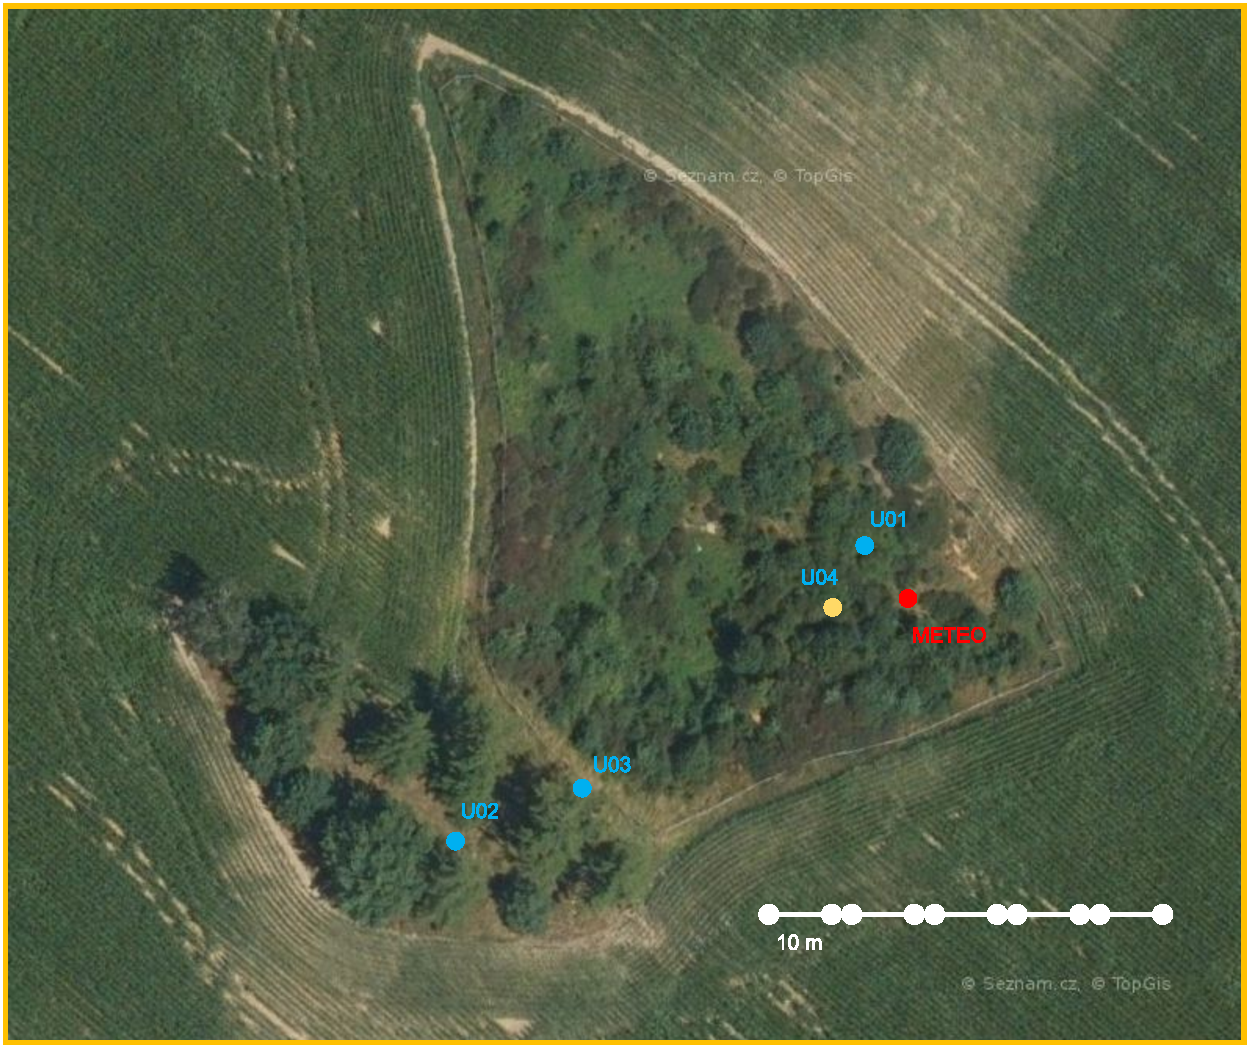
\includegraphics[width=0.62\linewidth]{fig/uhelna_meteo_mapa.pdf}
    \includegraphics[width=0.28\linewidth]{fig/meteo_stozar.pdf}
    \caption{Lokalita povrchového monitoringu v Uhelné a schéma stožáru meteostanice použitého pro kontinuální sběr meteorologických dat.}
    \label{fig:terenni-prace}
\end{figure}

Neméně důležitou součástí řešení byla laboratorní kolona, na níž bylo možné
testovat profilové sondy, řízení experimentů a numerický model za lépe
kontrolovaných podmínek než v terénu. V roce 2024 byla kolona zprovozněna pro
experimenty s volným odtokem a sledováním vlhkosti v čase. V roce 2025 byla
dále upravena tak, aby umožňovala i simulaci srážkových epizod, přesnější
měření dodané vody a následné testování 1D modelu s asimilací dat. Laboratorní
práce zároveň odhalily problémy s konzistencí čidel Odyssey a poskytly
podklady pro úpravy zpracování dat i kalibrace modelových parametrů.

Paralelně probíhal vývoj nekontaktního elektromagnetického čidla pro měření
vlhkosti v hluboké vadózní zóně. Tento směr měl zvýšit informační hodnotu
projektu tím, že by přinesl přímější data z hloubek mezi povrchem a hladinou
podzemní vody, kde běžný monitoring chybí. V roce 2024 byly prováděny
laboratorní experimenty s malými i většími prototypy a ČGS souběžně
připravovala suchý vrt pro jejich budoucí instalaci. Ukázalo se však, že
technická realizace čidla ve větší škále je podstatně náročnější, než se
předpokládalo. Tato větev projektu proto nebyla opuštěna, ale její role byla
postupně oslabena ve prospěch dokončení integrovaného predikčního systému.

\subsection{Vývoj softwaru a datové infrastruktury}
Na softwarové straně bylo nutné vyřešit dva související problémy: průběžný
sběr heterogenních dat a jejich uložení v podobě vhodné pro další výpočty a
vizualizaci. Zatímco v roce 2024 se řešilo především logování dat z terénní
stanice a z kolony, v roce 2025 byl vyvinut ucelenější datový tok založený
na knihovně \texttt{zarr-fuse} a službě Ingress. Jejich úkolem je přebírat
meteorologická data z veřejných online zdrojů, převádět je do jednotného
schématu a ukládat je ve formátu ZARR nad datovými strukturami
\texttt{xarray}. Vedle meteorologických dat jsou stejným principem
organizována i vlastní terénní měření a připravená schémata pro výstupy
simulací.

Výsledkem není pouze datový archiv, ale infrastruktura, která umožňuje
propojit měření, modelování a pozdější vizualizaci v jediném workflow. V
projektu tak vznikla samostatná vrstva, jejímž smyslem je oddělit získávání a
kuraci dat od samotného modelování. To je důležité zejména proto, že povrchový
model, hluboký model i jejich integrační vrstva pracují s časově a prostorově
závislými veličinami, které je potřeba konzistentně verzovat, doplňovat o
jednotky a zpřístupnit jak pro dávkové výpočty, tak pro kontrolní vizualizace.

\subsection{Numerické modelování a integrace}
Vývoj numerického jádra projektu probíhal postupně od dílčích modelů k jejich
integraci. V roce 2024 byl rozpracován 1D model proudění vody v nenasycené
zóně založený na Richardsově rovnici a na Kalmánově filtru, původně ve
variantě směřující k interpretaci profilových měření a laboratorních dat.
Vzhledem k nejistotám terénního měření a parametrů půdy se už tehdy ukázalo,
že bez průběžné asimilace dat a bez laboratorního testování nebude možné
spolehlivě odhadovat infiltrační tok do hlubší části systému.

V roce 2025 byl tento modelový základ výrazně rozšířen. Povrchový model byl
implementován nad simulátorem ParFlow, byly připraveny varianty pro popis
evapotranspirace od jednoduchého Priestleyho-Taylorova vztahu až po CLM a
byla zobecněna implementace Kalmánova filtru tak, aby bylo možné lépe
pracovat s náhodným stavem modelu a jeho kalibrací. Praktické testy na datech
z kolony vedly k závěru, že současná asimilace stavu a fitování materiálových
parametrů v jediném kroku je příliš citlivá na volbu procesního šumu. Z toho
důvodu byl přijat dvouúrovňový postup: asimilace slouží především ke korekci
aktuálního stavu modelu, zatímco kalibrace parametrů probíhá odděleně na
delším časovém úseku.

Souběžně ČGS připravovala a TUL přebírala GIS podklady pro hluboký
hydrogeologický model. Ten je budován nad jádrem MODFLOW~6 a jeho sestavení je
automatizováno pomocí skriptů, které převádějí vrstevnatý geologický model do
výpočetního rastru a materiálového gridu. Na této bázi vznikl i první
integrovaný výpočetní obraz, který propojuje povrchové modely s hlubokým
modelem a komunikační vrstvou pro paralelní výpočty. Ke konci roku 2025 tak
byly k dispozici všechny hlavní stavební bloky predikčního systému, i když
jejich úplné napojení na historická data a reálný hluboký model bylo ještě ve
stavu rozpracovanosti.

\subsection{Příspěvek České geologické služby}
Role České geologické služby byla v projektu dvojí. Na jedné straně
zajišťovala hydrologickou a hydrogeologickou interpretaci lokality Uhelná i
širšího kontextu hlubokých vrtů v České republice. Na straně druhé připravila
materiálové podklady, bez nichž by nebylo možné budovat hluboký model a
uvažovat o doplňkovém měření v hluboké vadózní zóně. ČGS proto realizovala
vrtné práce, technické zajištění a karotáže nových vrtů, průběžně sledovala
hladiny podzemní vody v okolí Uhelné a současně zpracovávala dosavadní
primární geologická data do 3D geologického modelu.

Z pohledu celého projektu je podstatné, že činnost ČGS nebyla jen dodávkou
podkladových map. Výběr vhodné lokality, interpretace režimních dat hladin
podzemní vody, návrh suchého vrtu i převod geologického modelu do vrstev pro
hydrogeologický výpočet tvoří nezbytnou část řetězce od terénního pozorování
ke kalibrovatelnému hlubokému modelu. Právě kombinace hustého lokálního
monitoringu v Uhelné a širšího srovnání s vrty pozorovací sítě ČHMÚ dává
projektu HLAVO obecnější význam přesahující jedinou studovanou lokalitu.

\begin{figure}[htb]
    \centering
    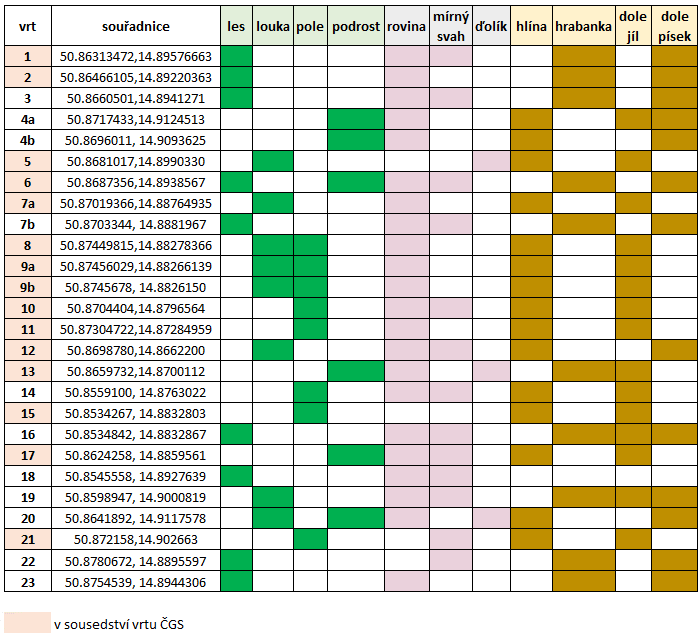
\includegraphics[width=0.8\linewidth]{fig/seznam_vrtu.png}
    \caption{Přehled vrtů a monitorovacích bodů využitelných pro geologický a hydrogeologický popis lokality Uhelná.}
    \label{fig:seznam-vrtu}
\end{figure}

\section{Rešerše podobných řešení}
\label{sec:reserse}
Pro projekt HLAVO jsou relevantní čtyři literární směry: provozní měření
půdní vlhkosti v terénu, fyzikální modelování infiltrace ve vadózní zóně,
interpretace hluboké perkolace a doplňování zásob podzemní vody a konečně
asimilace dat do procesních modelů. Starší přehledové práce zůstávají
užitečným metodickým východiskem \cite{Lekshmi2014,Cerny2009,Farthing_Ogden_2017},
ale literatura z let 2020 až 2025 ukazuje zřetelný posun od izolovaných
experimentů k víceškálovým monitorovacím a modelovacím sestavám, které mají
sloužit přímo pro provozní interpretaci infiltrace a dotace podzemních vod.

V oblasti monitoringu půdní vlhkosti se recentní literatura soustředí méně na
samotný princip senzoru a více na kvalitu instalace, kalibraci, reprezentativnost
měření a kombinaci různých prostorových měřítek. Praktický význam má zejména
standardizace instalace a provozu profilových čidel v nenarušené půdě
\cite{CaldwellEtAl2022}. Současně se prosazují přístupy, které doplňují bodová
\textit{in situ} měření o plošněji reprezentativní metody, například
cosmic-ray neutron sensing pro přechod mezi profilem a polem
\cite{RascheEtAl2024CRNS}, případně nové distribuované postupy založené na
optických vláknech a nepřímém snímání dynamiky vlhkosti ve vadózní zóně
\cite{ShenEtAl2024Fiber}. Přehled \textcite{Duarte_Hernandez_2024} potvrzuje,
že právě kombinace více typů pozorování je dnes považována za vhodný směr
v lokalitách s výraznou prostorovou variabilitou a omezenou možností přímého
mapování infiltrace.

Numerické jádro obdobných řešení zůstává i v recentní literatuře založeno na
Richardsově rovnici a na explicitním popisu proudění ve variably saturovaném
prostředí. Vedle klasických numerických přístupů se však nově rozvíjejí
inverzní a hybridní metody, které mají lépe využít řídká nebo nepravidelná
data. \textcite{Bandai_Ghezzehei_2021} ukazují, že physics-informed neuronové
sítě lze použít k odhadu konstitutivních vztahů i toků přímo z časových řad
vlhkosti, aniž by se rezignovalo na fyzikální omezení úlohy. Podobně
\textcite{LanEtAl2024PIDL} rekonstruují infiltrační chování z omezených dat
pomocí fyzikálně informovaného hlubokého učení. V širším kontextu
\textcite{ShenEtAl2023Differentiable} popisují nástup diferenciovatelných
modelů, které propojují procesně založené rovnice s metodami strojového učení.
Pro HLAVO je podstatné, že recentní směr nevede k nahrazení fyzikálního modelu
čistě datovou aproximací, ale k přesnějšímu napojení měření na fyzikálně
interpretovatelný model infiltrace.

Samostatnou linií je interpretace hluboké vadózní zóny a odhadu dotace
podzemních vod. Zde recentní práce zdůrazňují, že mezi povrchovým impulzem a
odezvou zvodně může působit významná retence, zpoždění a nelinearita, kterou
nelze dostatečně vystihnout jednoduchým převodem srážka--infiltrace. Přehled
\textcite{HeEtAl2024DeepVadoseReview} shrnuje, že v hluboké vadózní zóně
rozhoduje vrstevnatost, preferenční proudění i sezónní stav zásob. Polem
podložené studie pak ukazují, že z časových řad půdní vlhkosti lze odhadovat
toky ve vadózní zóně, ale jen při dobré znalosti lokální struktury prostředí
\cite{SchueblEtAl2023}; heterogenita může zásadně změnit efektivitu řízené i
přirozené dotace \cite{ZhouEtAl2023VadoseMAR}; a významnou roli hraje také
hluboké akumulační zpoždění mezi infiltrací a skutečnou dotací zvodně
\cite{LiEtAl2023LoessRecharge,BenitezNelsonEtAl2025}. V tomto směru jsou pro
HLAVO stále inspirativní i práce O.~Dahana, které zavedly dlouhodobý monitoring
hluboké vadózní zóny jako nástroj ochrany a interpretace podzemních vod
\cite{Dahan_McDonald_Young_2003,Dahan_Talby_Yechieli_2009,Dahan2020}.

Takové modely mají praktickou hodnotu teprve tehdy, když dokážou průběžně
využívat aktuální data. Ensemble Kalman filter a jeho hydrologické varianty
zůstávají základním rámcem \cite{Evensen2003}, přičemž starší aplikace již
ukázaly použitelnost pro procesně založené modely povrchového a podpovrchového
proudění \cite{Camporese2009,Carlo2018}. Recentní literatura jde dále směrem
k asimilaci více typů pozorování současně. \textcite{LiEtAl2025JointAssimilation}
ukazují, že společná asimilace plošně reprezentativních dat o půdní vlhkosti a
hladin podzemní vody zlepšuje odhad zásob vody i rozdělení toků v systému.
Právě zde je nejbližší vazba na cíle HLAVO: nestačí pouze simulovat infiltraci,
ale je třeba průběžně korigovat stav modelu podle reálných profilových a
hydrogeologických pozorování.

Z recentní rešerše tedy plyne, že jednotlivé stavební kameny projektu mají v
současné literatuře dobrou oporu, avšak většinou jako dílčí řešení. Literatura
nabízí buď pokročilý monitoring půdní vlhkosti, nebo samostatné modely
vadózní zóny, nebo asimilaci vybraných datových proudů. Méně běžné je jejich
spojení do jednoho provozně použitelného řetězce, který by v konkrétní
lokalitě kombinoval hustou síť profilových měření, meteorologická data,
fyzikálně interpretovatelný infiltrační model a návaznou predikci hladin
podzemní vody. Právě tuto integrační mezeru projekt HLAVO adresuje.

\section{Vlastnosti výsledku: software HLAVO a funkční vzorek integrace}
%AGENT: zatím zde skončit a dále neřešit
Tato sekce má být jádrem zprávy a současně má částečně fungovat jako český
rámcový návod k použití systému HLAVO. Text proto nemá být jen seznamem
komponent, ale i vysvětlením jejich role, vstupů, výstupů a vazeb.

\subsection{Síť měření vlhkosti}

Zde bude stručně popsána použitá měřicí technika, rozmístění profilů a typ
výstupních dat. Ve větším detailu je potřeba rozepsat praktické otázky
instalace, napájení, servisu a dlouhodobého provozu sítě profilových měření,
protože tyto informace nejsou plně popsány v technické softwarové
dokumentaci.

\begin{figure}[htb]
    \centering
    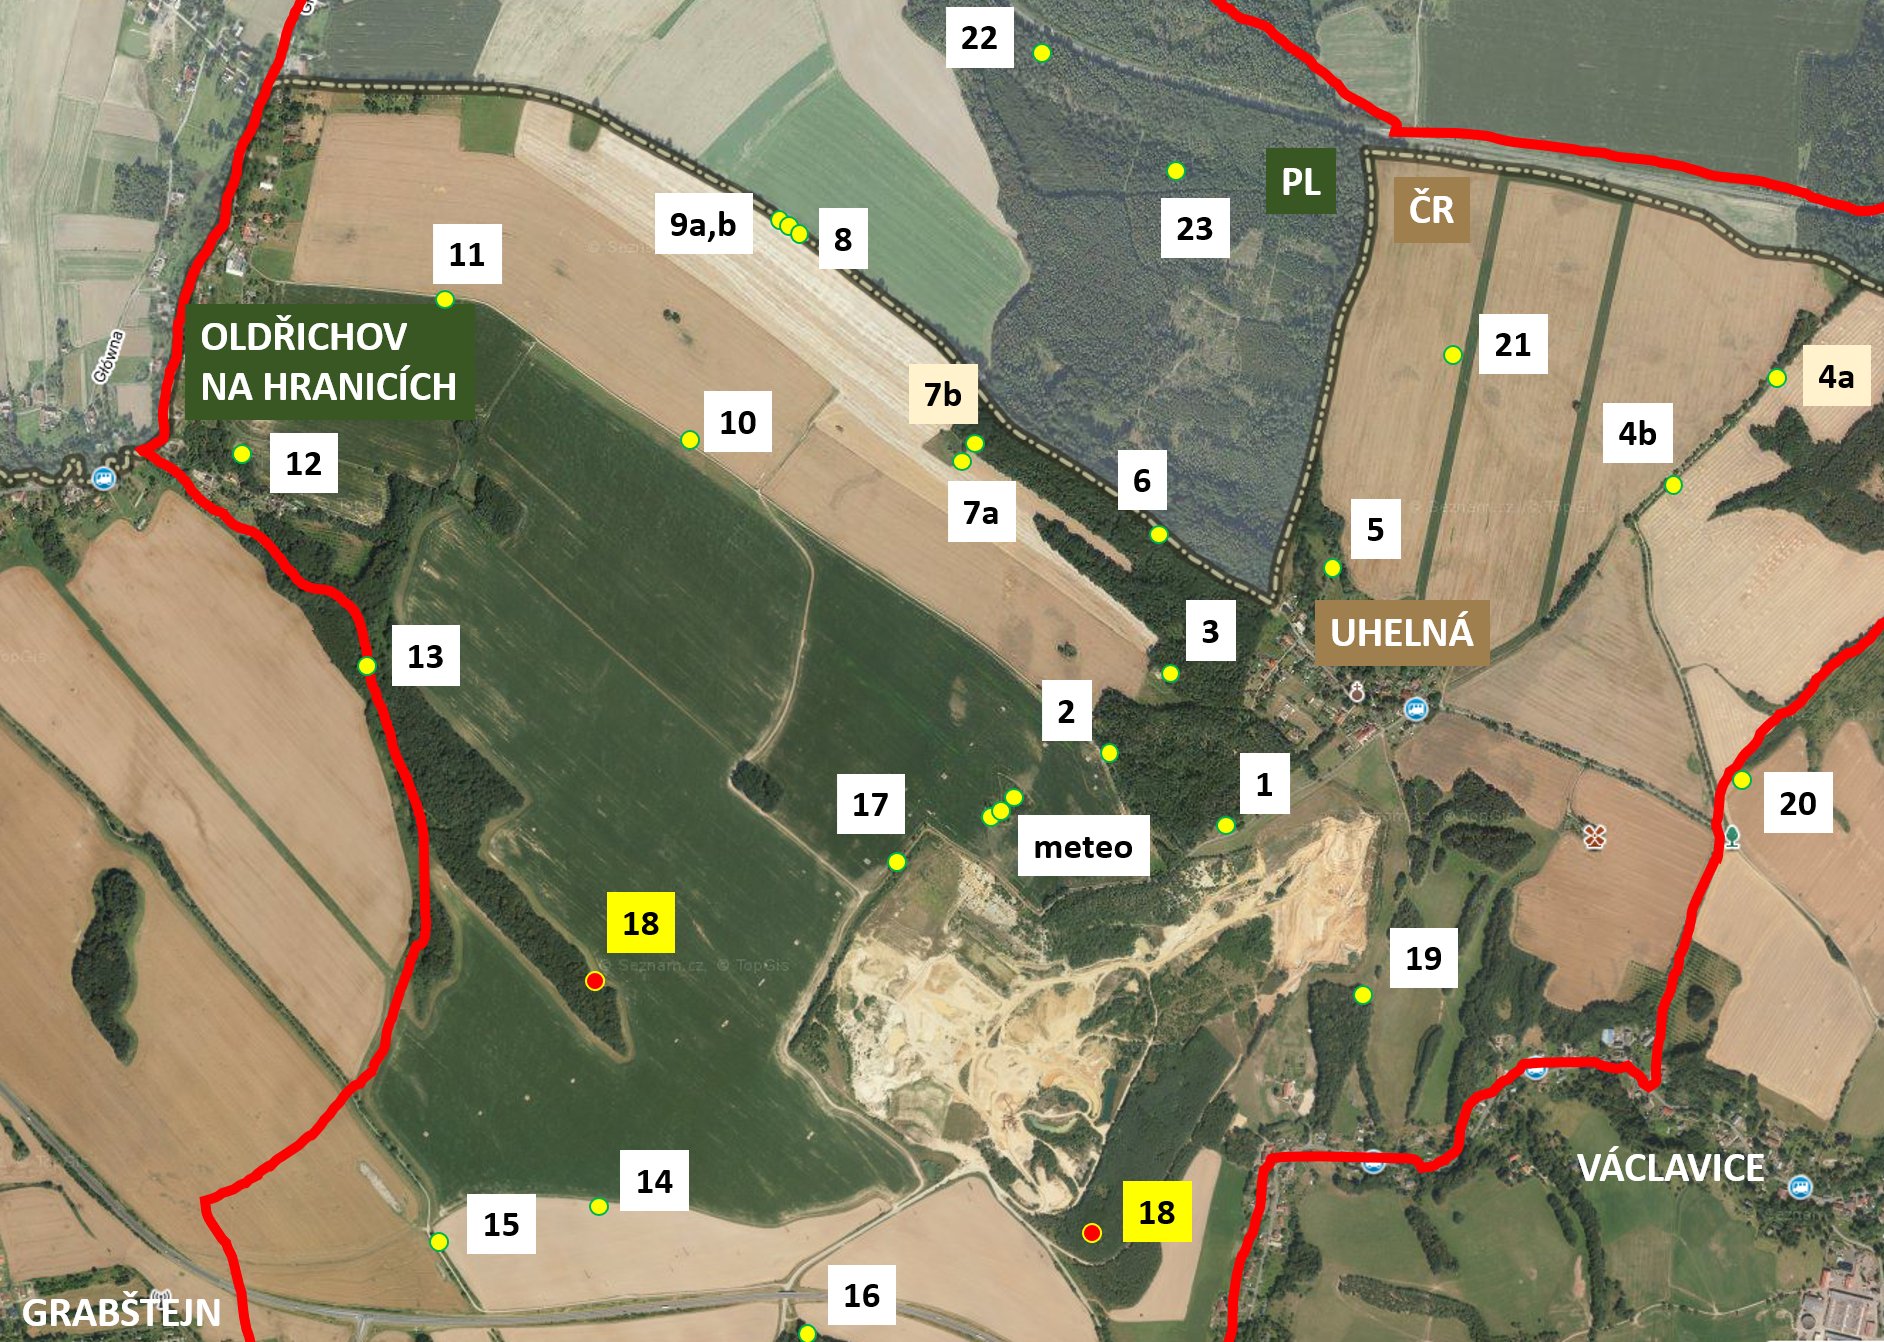
\includegraphics[width=0.58\linewidth]{fig/uhelna_sondy.png}
    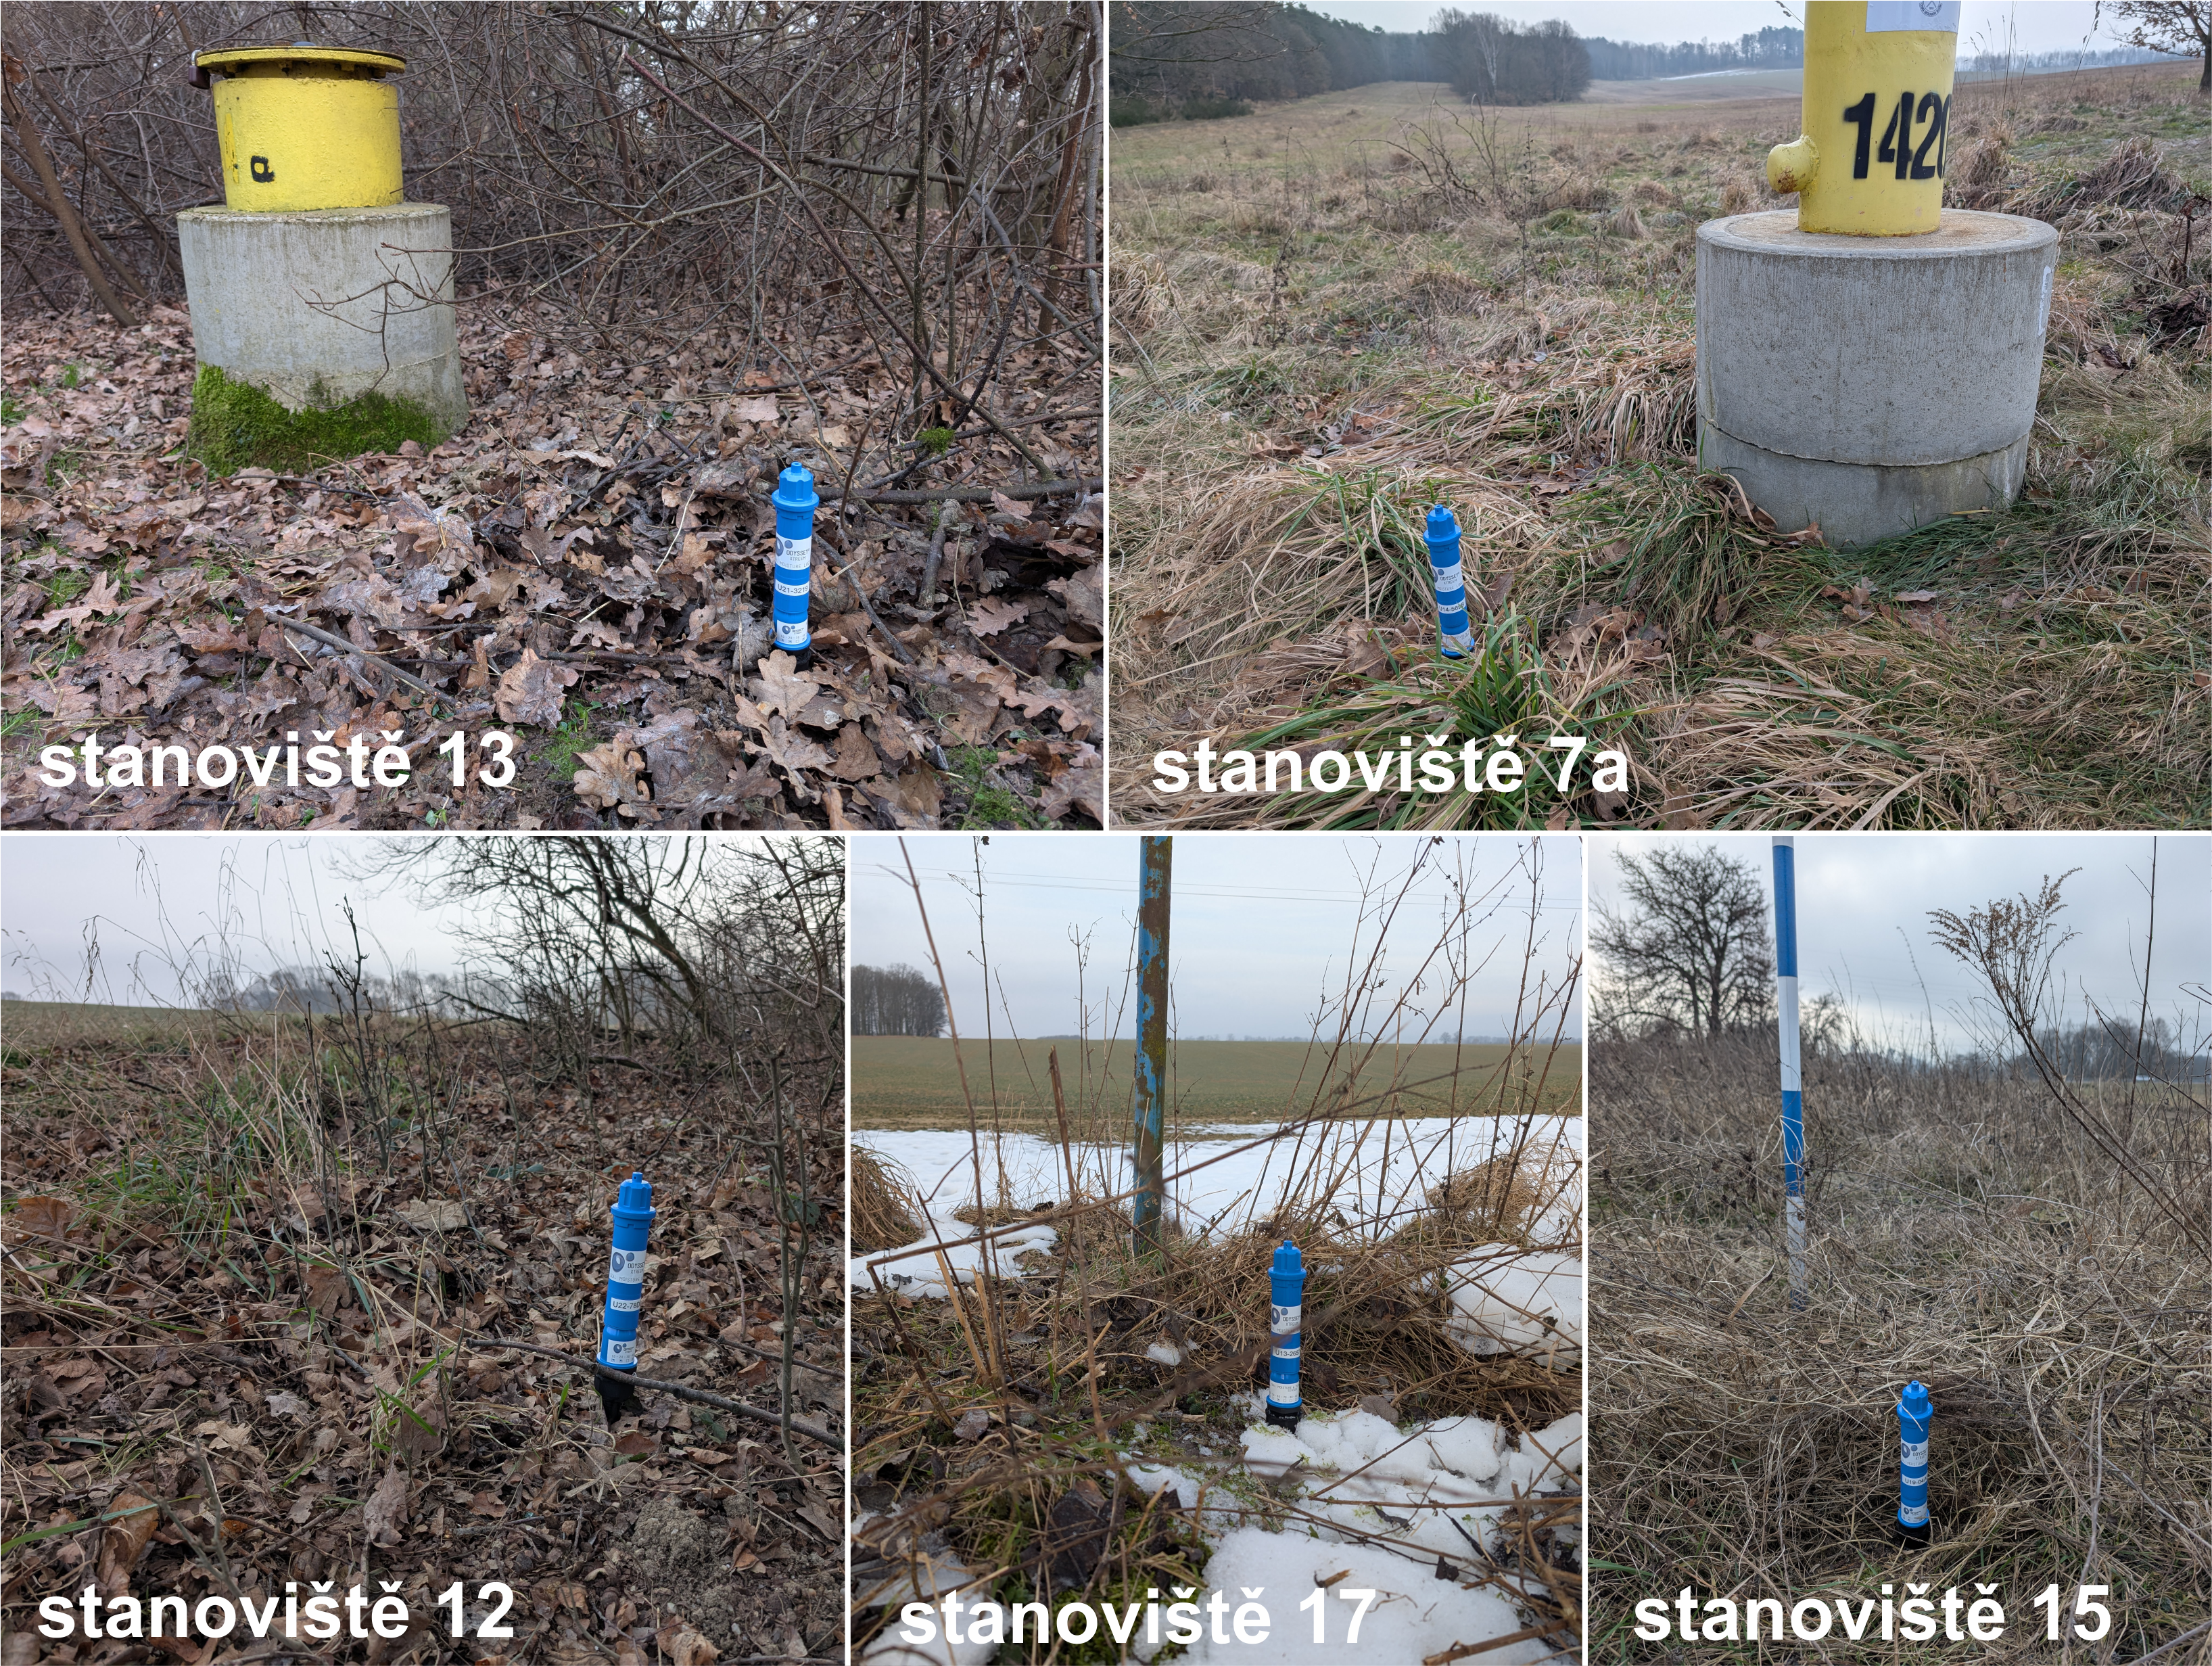
\includegraphics[width=0.34\linewidth]{fig/instalace_site.png}
    \caption{Pracovní výběr k popisu sítě měření vlhkosti: rozmístění profilových sond a detail instalace v terénu.}
    \label{fig:sit-vlhkosti}
\end{figure}

\subsection{Automatický sběr meteorologických dat}

Zde bude popsán sběr dat z veřejných zdrojů a jejich role pro výpočet
evapotranspirace a povrchového modelu.

\subsection{Organizace a ukládání dat}

Zde bude vysvětlena role datových schémat, knihovny \texttt{zarr-fuse},
využití \texttt{xarray} a formátu ZARR
\cite{Xarray_HoyerHamman2017,ZarrPython_Zenodo2025}. Pro detailní technické
informace bude možné odkázat na repozitář HLAVO \cite{HLAVO_GitHub}.

\begin{figure}[htb]
    \centering
    
\includegraphics[width=0.95\linewidth]{fig/zarr_fuse_ingress.pdf}
    \caption{Pracovní schéma datového toku: sběr, konverze a ukládání dat v infrastruktuře HLAVO.}
    \label{fig:zarr-ingress}
\end{figure}

\begin{figure}[htb]
    \centering
    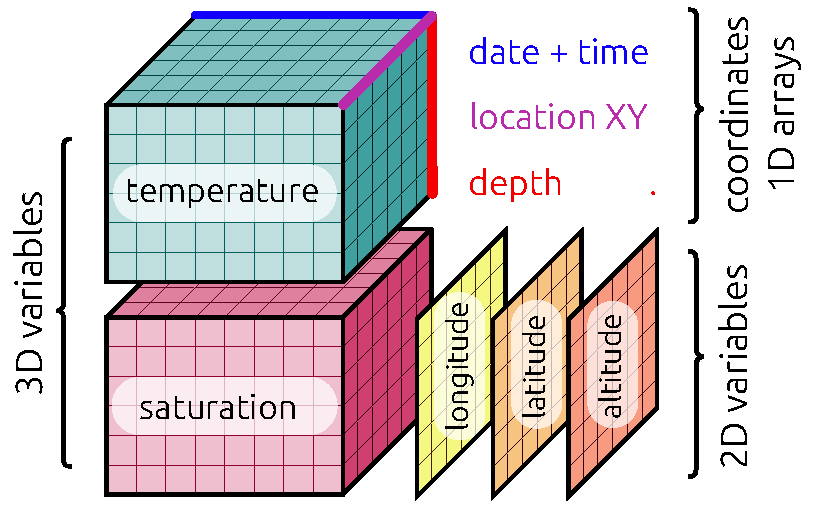
\includegraphics[width=0.72\linewidth]{fig/hlavo_example.pdf}
    \caption{Pracovní ukázka struktury datasetu, která může doprovodit stručný popis datových schémat a vazby na repozitář HLAVO.}
    \label{fig:hlavo-example}
\end{figure}

\subsection{Kalmánův filtr a povrchový model}

Zde bude popsáno propojení Richardsova modelu, meteorologických vstupů a
asimilace měření vlhkosti. Vhodné je zachovat věcnou úroveň podobnou zprávě
za rok 2025.

\begin{figure}[htb]
    \centering
    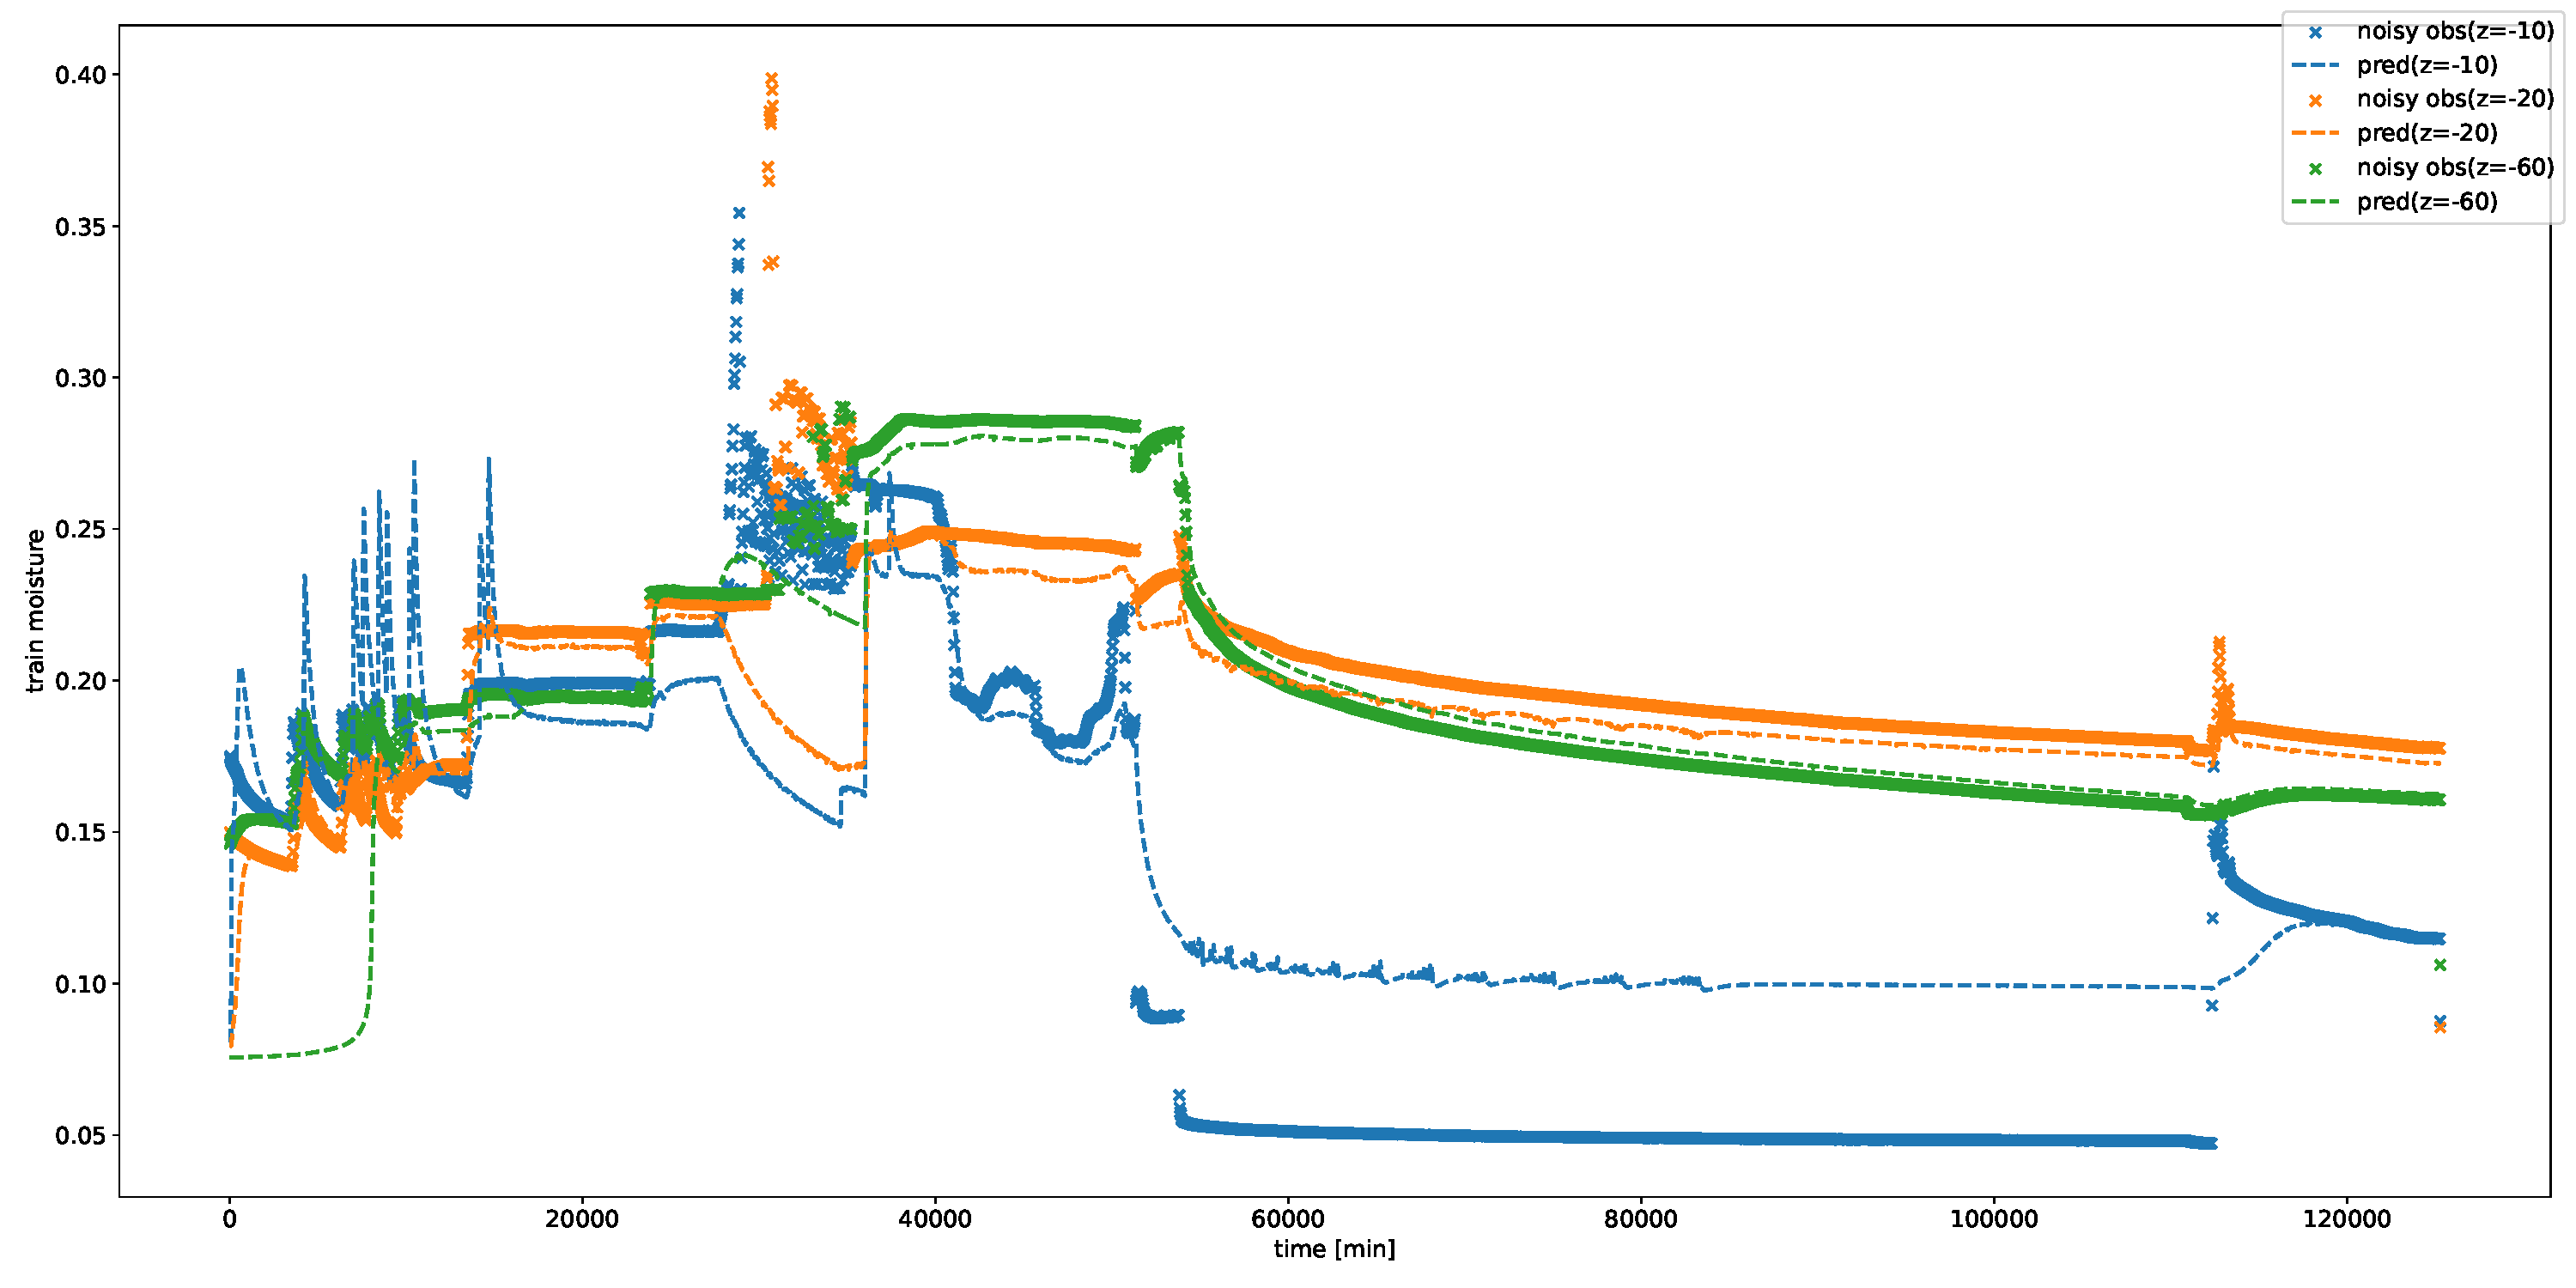
\includegraphics[width=0.88\linewidth]{fig/kalman_kolona.pdf}
    \caption{Pracovní obrázek k části o asimilaci dat: ukázka aplikace 1D modelu s Kalmánovým filtrem na datech z kolony.}
    \label{fig:kalman-kolona}
\end{figure}

\subsection{Hluboký model vadózní zóny}

Zde bude popsána konstrukce hlubokého modelu z GIS podkladů a jeho role v
predikci hladin podzemní vody. Pro základní rámec lze odkázat na MODFLOW 6
\cite{MODFLOW6_Framework_Hughes2017}.

\begin{figure}[htb]
    \centering
    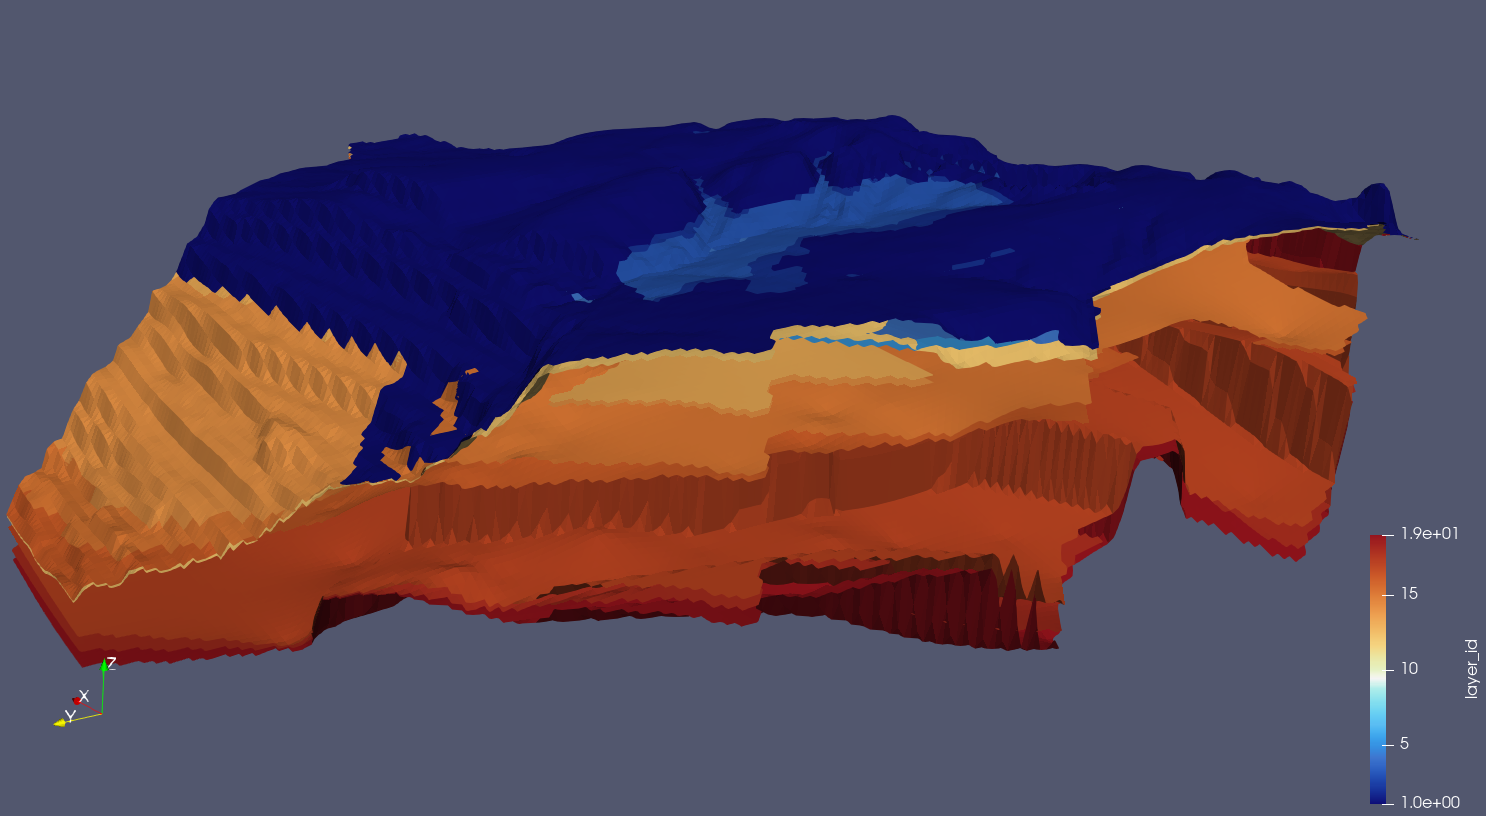
\includegraphics[width=0.95\linewidth]{fig/layers_large_domain.png}
    \caption{Pracovní obrázek k hlubokému modelu: vrstvy a rozsah modelované oblasti odvozené z GIS podkladů.}
    \label{fig:deep-model}
\end{figure}

\subsection{Integrovaný výpočetní systém}

Zde bude popsáno, jak na sebe navazují měření, datové úložiště, povrchový
model a hluboký model. Důležité je oddělit to, co je plně funkční, od toho,
co je ve stavu prototypu nebo částečné integrace.

\begin{figure}[htb]
    \centering
    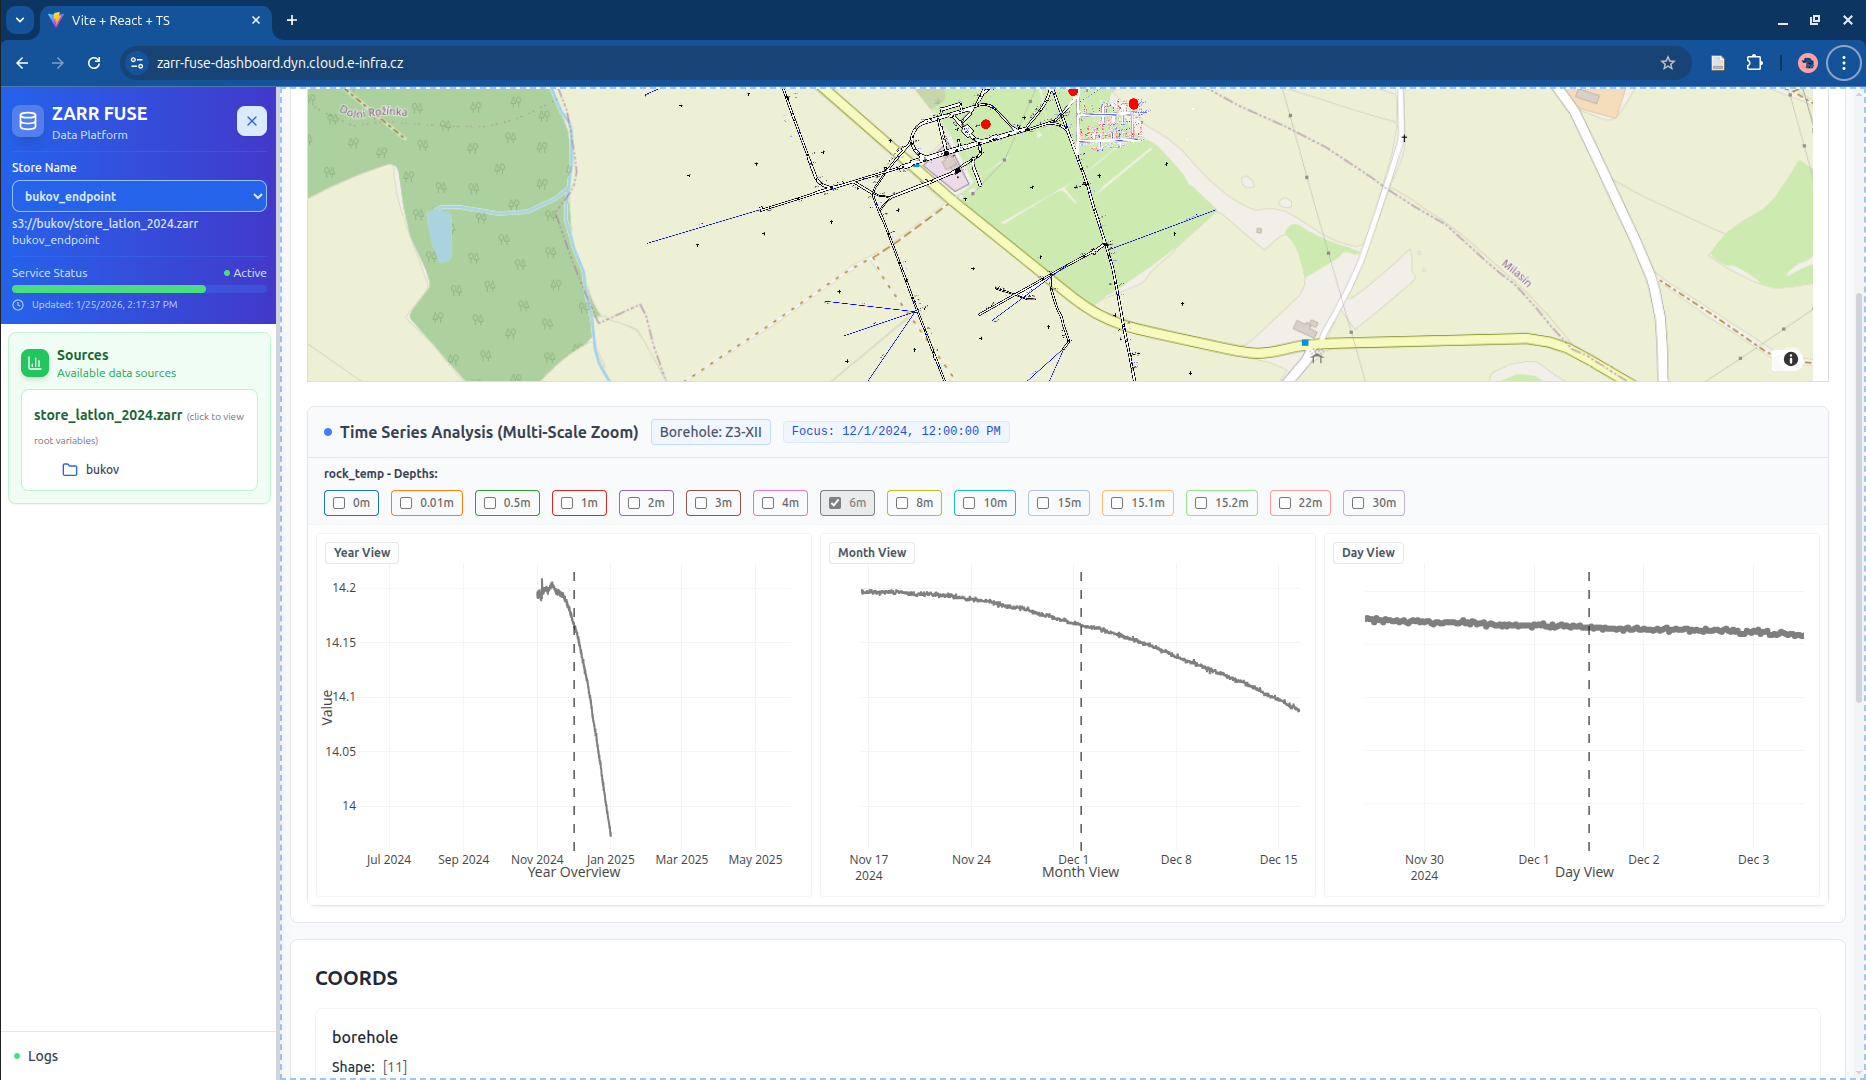
\includegraphics[width=0.95\linewidth]{fig/dashboard.png}
    \caption{Pracovní ukázka vizualizační vrstvy systému HLAVO pro měřená a simulovaná data.}
    \label{fig:dashboard}
\end{figure}

\section{Aplikace na lokalitu Uhelná}

Tato sekce bude hlavní případovou studií. Je vhodné ji vystavět tak, aby na
jednom místě shrnula vstupní data, konfiguraci systému pro lokalitu Uhelná a
praktické zkušenosti z nasazení.

\subsection{Meteodata a jejich zdroje}

Zde bude uvedeno, jaké meteorologické zdroje byly použity, jak jsou do
systému přiváděny a jaké mají časové a věcné pokrytí.

\subsection{Síť profilových měření}

Zde bude popsáno rozmístění sond, typy sond, způsob instalace a praktické
poznatky z provozu a údržby.

\begin{figure}[htb]
    \centering
    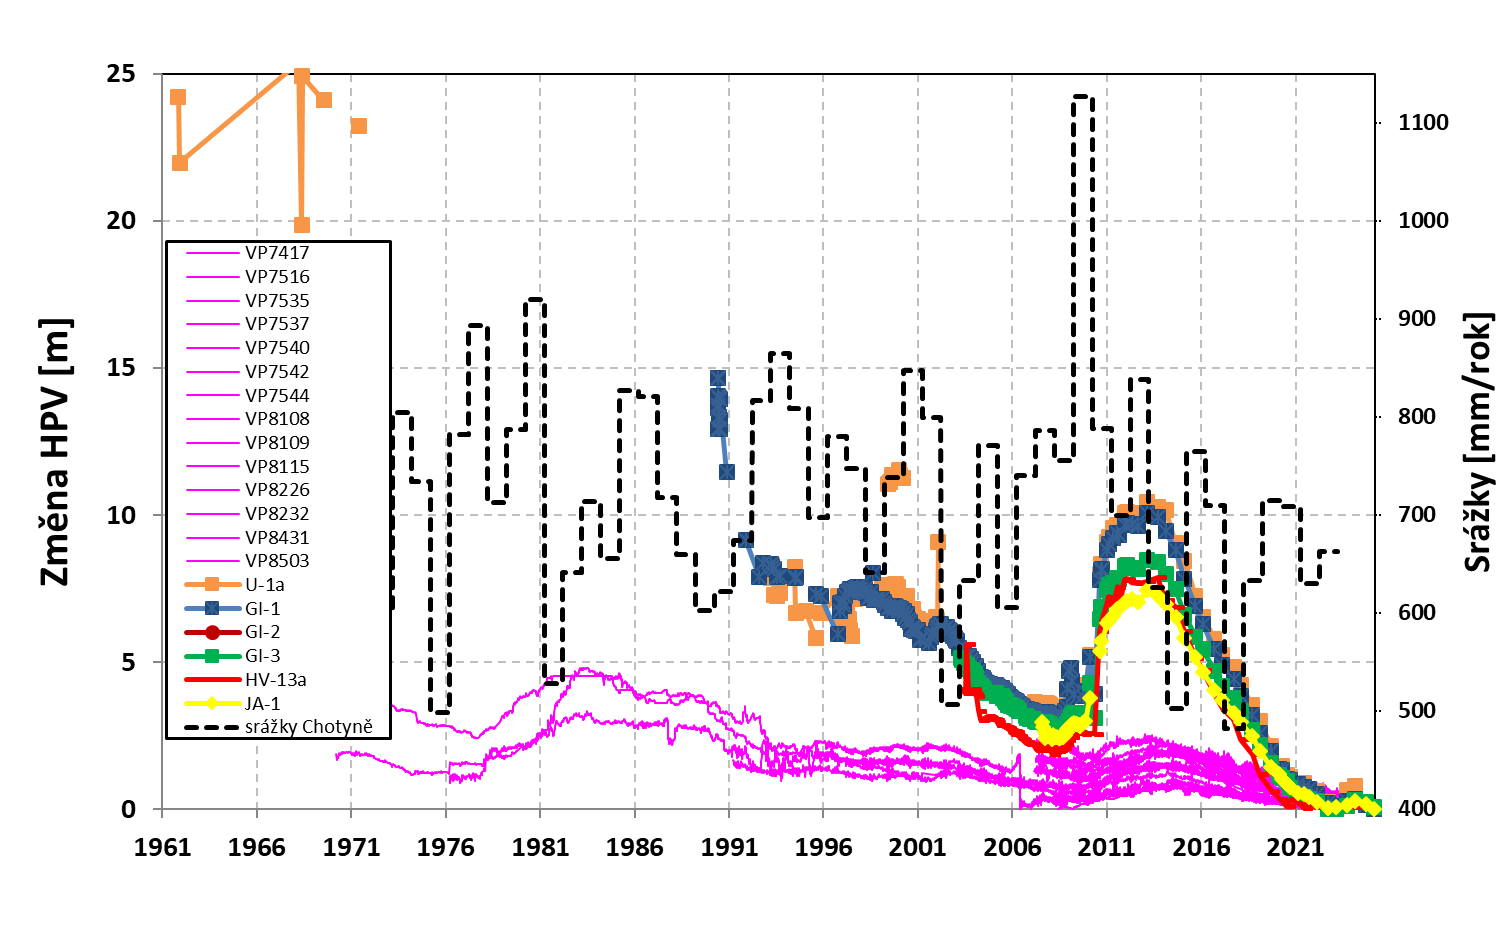
\includegraphics[width=0.92\linewidth]{fig/cgs_monitoring_uhelna_chmu.png}
    \caption{Pracovní podklad pro aplikaci na Uhelnou: přehled monitoringu hladin podzemních vod a vazba na meteorologické podklady.}
    \label{fig:cgs-monitoring-uhelna}
\end{figure}

\subsection{Příprava modelu z GIS dat}

Zde bude vysvětlena role vrstev dodaných ČGS, jejich zpracování a převod do
výpočetní podoby.

\subsection{Hladiny podzemních vod a kalibrace}

Zde bude popsáno, která data o hladinách podzemních vod byla k dispozici,
jak sloužila nebo budou sloužit pro kalibraci a jaká omezení z toho plynou.

\begin{figure}[htb]
    \centering
    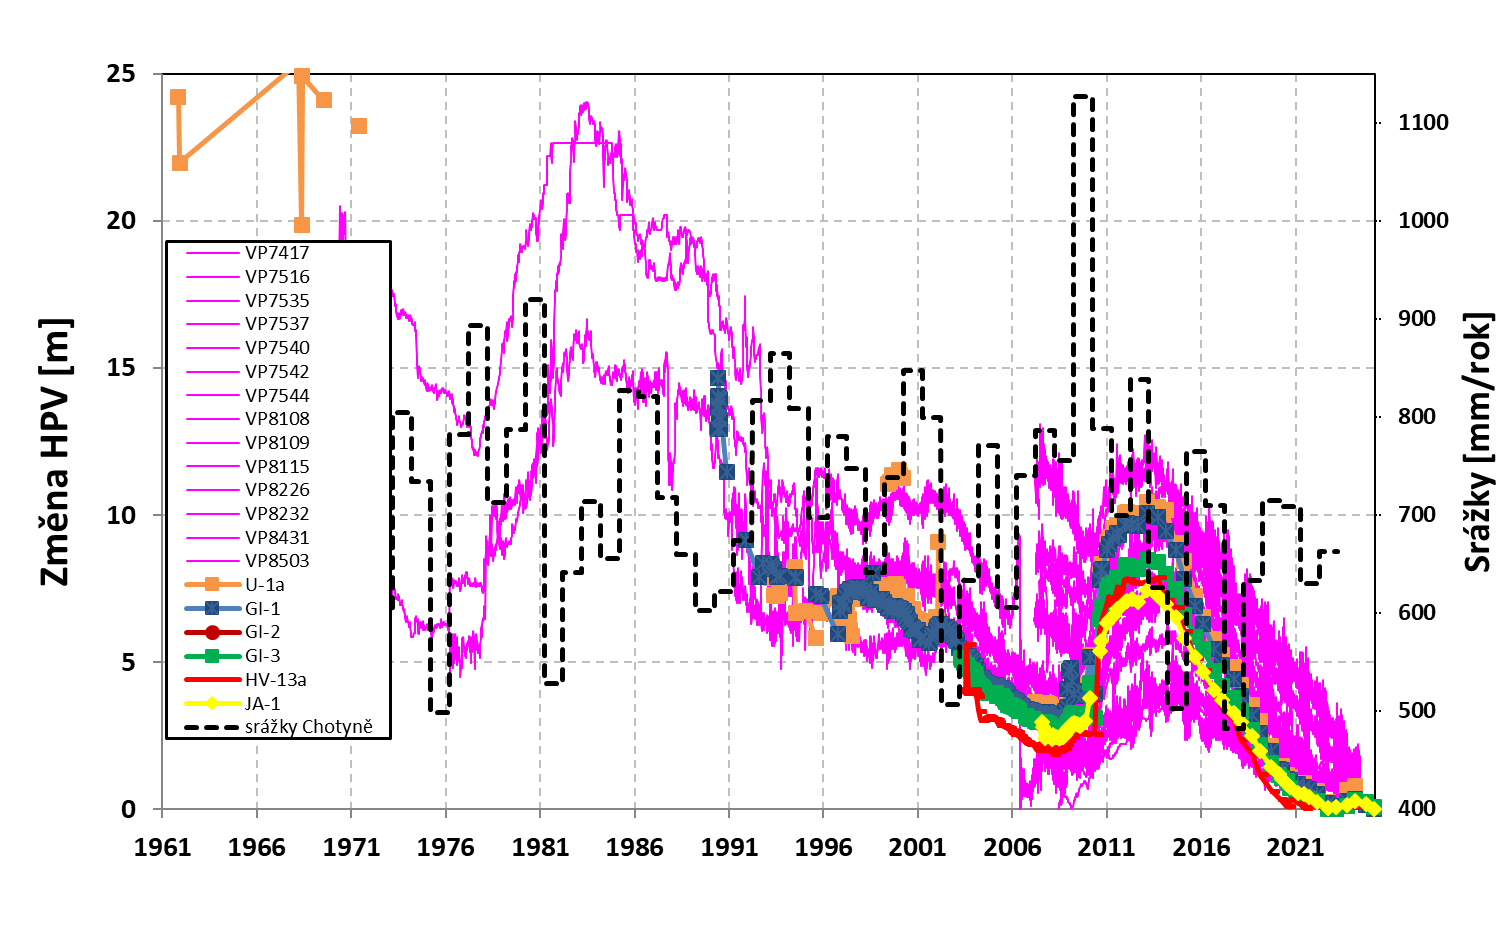
\includegraphics[width=0.92\linewidth]{fig/cgs_monitoring_uhelna_chmu_5x.png}
    \caption{Pracovní detail k části o kalibraci hlubokého modelu na lokalitě Uhelná.}
    \label{fig:cgs-monitoring-uhelna-detail}
\end{figure}

\subsection{Ukázka současného použití systému}

Zde je prostor pro jednu až dvě reprezentativní ukázky datového toku,
vizualizace nebo výsledku modelování pro lokalitu Uhelná.

\section{Aplikace na jinou lokalitu}

Tato sekce má vysvětlit přenositelnost výsledku mimo Uhelnou. Má jít o
obecný popis kroků pro zatím neupřesněnou lokalitu v prostředí České
křídové tabule. Měla by jasně říci, co lze přenastavit snadno a co je
hlavním omezujícím faktorem.

\subsection{Snadno přenositelné části systému}

Sem patří zejména konfigurace zdrojů meteorologických dat, datová schémata a
postupy pro sběr a zobrazení dat.

\subsection{Podmínky pro nové profilové měření}

Zde bude popsáno, jak závisí návrh měřicí sítě na typu povrchu, půdy a
praktických možnostech instalace.

\subsection{Požadavky na geologické a hydrogeologické podklady}

Zde bude vysvětleno, že hlavní překážkou přenosu systému není samotný
software, ale spolehlivá znalost geologie a dat pro kalibraci hlubokého
modelu.

\subsection{Doporučený postup nasazení}

Zde vznikne stručný návod, v jakém pořadí postupovat při aplikaci systému na
novou lokalitu.

\section{Závěr}

Závěr má shrnout, co projekt skutečně přinesl z pohledu metodiky,
softwarového řešení, terénního ověření a připravenosti pro další použití.
Současně je vhodné otevřeně uvést, které části systému byly dotaženy do
prakticky použitelné podoby a které zůstávají podmíněny doplněním dat nebo
další kalibrací.

V závěru bude také vhodné explicitně oddělit:

\begin{itemize}
    \item přínosy projektu pro MŽP a aplikační praxi,
    \item technické limity současného řešení,
    \item doporučení pro další nasazení nebo navazující vývoj.
\end{itemize}

\printbibliography[heading=bibintoc,title={Použitá literatura}]

\end{onehalfspacing}
\end{document}
